% workaround for problem with white text if notes are enabled
% http://tex.stackexchange.com/questions/232168/normal-text-is-invisible-when-using-beamer-with-notes-and-xelatex
\def\pgfsysdriver{pgfsys-dvipdfm.def}

\documentclass{beamer}

\usetheme{metropolis}
\setbeamercolor{normal text}{bg=white} % white background instead of black!2

\usepackage{pgfpages}
\setbeameroption{show notes on second screen}


\usepackage{ifxetex}
\ifxetex
  \usepackage{polyglossia}
  \setmainlanguage{russian}
  \setotherlanguage{english}

  % workaround for "Package polyglossia Error: The current roman font does not contain the Cyrillic script!"
  \newfontfamily\cyrillicfonttt{Fira Sans}
\else
  \usepackage[T2A]{fontenc}
  \usepackage[utf8]{inputenc}
  \usepackage[english,russian]{babel}

  % workaround for "Package hyperref Warning: Glyph not defined in PD1 encoding"
  \hypersetup{unicode=true}
\fi

\newcommand{\eng}[1]{
  \ifxetex
    {\textenglish{#1}}
  \else
    {\foreignlanguage{english}{#1}}
  \fi
}

% numbers formating: \num{123456}
\usepackage{numprint}
\newcommand{\num}[1]{\numprint{#1}}
  \npthousandsep{\,}
  \npthousandthpartsep{}
  \npdecimalsign{,}

\newcommand{\pcnum}[1]{\ensuremath{\mathtt{#1}}}
\newcommand{\bin}[1]{\pcnum{#1}_2}
\newcommand{\hex}[1]{\pcnum{#1}_{16}}

\hypersetup{pdfauthor={Владимир Парфиненко}}
\title{Основы программирования}
\subtitle{Лекция № 2, XX февраля 2016 г.}
\date{}
\institute{
  \vspace{1em}
  \centering
  \parbox{0.8\textwidth}{
    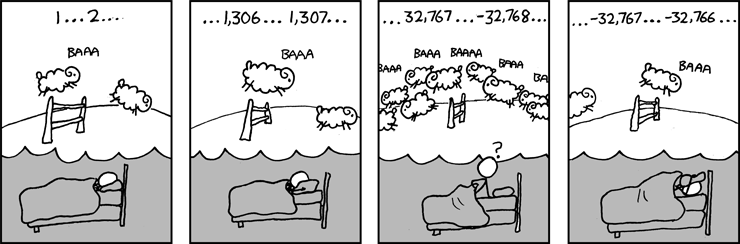
\includegraphics[width=\linewidth]{xkcd_cant_sleep}
    \par
    \raggedleft\tiny\url{http://xkcd.com/571}
  }
}


\begin{document}

\begin{frame}[plain]
  \titlepage
\end{frame}

\begin{frame}{Знакомство}

  Я~--- Владимир Парфиненко,

  \begin{itemize}
    \item бакалавр физики (ФФ), магистр математики (ММФ),
    \item профессиональный программист (Excelsior),
    \item регулярно чему-то учу (ФФ, АФТИ, ЛШ ФМШ).
  \end{itemize}

  Контакт:
  \href{mailto:vladimir.parfinenko@gmail.com}{vladimir.parfinenko@gmail.com}

\end{frame}

\section{Представление целых чисел}
\note{
  Порассуждать о том, как с помощью двух ламп можно представить числа от 0 до 3
}

\begin{frame}{Двоичная система счисления}

  Самый простой метод записи чисел, использующий только две цифры: 0 и 1.
  \note{комьютеру легко работать с такими числами\\}

  С помощью $n$ \emph{позиций} можно записать $2^n$ чисел.
  \note{Суффикс $x_{10}$ будем опускать\\}
  \begin{align*}
    \bin{000} &= 0, &\qquad \bin{100} &= 4, \\
    \bin{001} &= 1, &\qquad \bin{101} &= 5, \\
    \bin{010} &= 2, &\qquad \bin{110} &= 6, \\
    \bin{011} &= 3, &\qquad \bin{111} &= 7.
  \end{align*}
\end{frame}

\begin{frame}{Двоичная система счисления}

  Перевод из двоичной в десятичную:
  \begin{gather*}
    \bin{11001} = \mathbf{1} \cdot 2^4 + \mathbf{1} \cdot 2^3 +
                  \mathbf{0} \cdot 2^2 + \mathbf{0} \cdot 2^1 +
                  \mathbf{1} \cdot 2^0 = 16 + 8 + 1 = 25.
  \end{gather*}
  Перевод из десятичной в двоичную:
  \note{сказать про обратный порядок\\}
  \begin{align*}
    25 &= 2 \cdot 12 + \mathbf{1}, \\
    12 &= 2 \cdot 6 + \mathbf{0}, \\
    6 &= 2 \cdot 3 + \mathbf{0}, \\
    3 &= 2 \cdot 1 + \mathbf{1}, \\
    1 &= 2 \cdot 0 + \mathbf{1}.
  \end{align*}

\end{frame}

\begin{frame}{Числа в памяти компьютера}

  1 \emph{байт} состоит из 8 \emph{бит} и может кодировать $2^8 = 256$
  различных чисел.
  \note{пояснить, что байт - минимальная ячейка памяти, которую компьютер может
  читать/писать\\}

  Например, для кодирования числа 337 нужно, как минимум, 2 байта:
  \begin{gather*}
    \underbrace{\pcnum{00000001}}_{\text{биты } 15 \ldots 8}
    \underbrace{\pcnum{01010001}}_{\text{биты } 7 \ldots 0}
  \end{gather*}

  Предельные значения:
  \begin{itemize}
    \item 8 бит: $0 \ldots \num{255}$,
    \item 16 бит: $0 \ldots \num{65535}$,
    \item 32 бита: $0 \ldots \num{4294967295}$,
    \item 64 бита: $0 \ldots \num{18446744073709551615}$.
  \end{itemize}
\end{frame}

\begin{frame}{Шестнадцатеричная система счисления}

  Цифры: $\pcnum{0}, \pcnum{1}, \pcnum{2}, \pcnum{3}, \pcnum{4}, \pcnum{5},
  \pcnum{6}, \pcnum{7}, \pcnum{8}, \pcnum{9}, \pcnum{A}, \pcnum{B}, \pcnum{C},
  \pcnum{D}, \pcnum{E}, \pcnum{F}$.

  Перевод в двоичную и обратно через тетрады (по 4 бита):
  \begin{gather*}
    \bin{101011100} = \pcnum{\{0001\}\{0101\}\{1100\}} = \hex{15C}.
  \end{gather*}

  «Понятная» запись констант:
  \begin{itemize}
    \item 8 бит: диапазон чисел $\hex{0} \ldots \hex{FF}$,
    \item 32 бита: диапазон чисел $\hex{0} \ldots \hex{FFFFFFFF}$,
    \item $\texttt{0xDEADBEEF}, \texttt{0xCAFEBABE}, \texttt{0xCDCDCDCD},
      \ldots$
      \note{отладочная печать, Java-класс файл, неинициализированная память\\}
  \end{itemize}

\end{frame}

\begin{frame}{Знаковые числа}

  Отдельной памяти под знак нет, поэтому нужно упаковывать его в те же 8 (16,
  32, \ldots) бит.

  Заметим, что компьютер выполняет сложение и вычитание по модулю,
  соответствующему размеру числа. Рассмотрим сложение $\hex{FF} + \hex{01}$:
  \begin{gather*}
    \begin{array}{r}
    +
      \begin{array}{r}
        \pcnum{11111111} \\
        \pcnum{00000001} \\
      \end{array} \\
      \hline
      \begin{array}{r}
        \pcnum{1}\underbrace{\pcnum{00000000}}_{8 \text{ бит}}
      \end{array}
    \end{array}
  \end{gather*}

  С точки зрения компьютера $(\hex{FF} + \hex{01}) \mod 2^8 = \hex{00}$.

  То есть $X + 1 = 0$. Чему равно $X$?

\end{frame}

\plain{Конец второй лекции}

\end{document}
